  %!TEX root = main.tex
\paragraph{Argument optimal solution}
\paragraph{Numerical Optimization Description}
    \begin{itemize}
        \item Describe IPOP methd and cite BOCOP.
        \item Cite gitHub repository.
    \end{itemize}
\paragraph{Interpretations of a optimal solution}

    According to the WHO Strategic Advisory Group of Experts (SAGE) on
Immunization Working Group on COVID-19 Vaccines modeling questions
presented in \cite{sage2020}, our model is capable to explore the
following scenarios:
    \subsection*{Vaccine profile}
    Vaccination policies according to different profiles, namely:
    \begin{itemize}
      \item
          efficacy
          $\epsilon = \{\num{0.1}, \num{0.2}, \cdots  \num{0.9} \}$ .
      \item
        vaccine induced immunity
        $
          \delta_V ^{-1}=
            \{\SI{0.5}{year},
              \SI{1.0}{year}, \cdots, \SI{}{lifelong}
            \}.
        $
    \end{itemize}


  \subsection*{Coverage}
    We obtained optimal vaccination policies with coverage profiles at
    $$
      x_{coverage} =
        \{
          20\%, 50\%, 80\%
        \}.
    $$
  \subsection*{Time horizon}
  Plausible scenarios at time horizon
  $
    T= \{ \SI{1}{year}, \SI{2}{year}, \SI{10}{year} \}.
  $

    To fix ideas,  we display in \Cref{fig:lifelongvaccinationpolicies} the
counterfactual scenario regarding no intervention, constant vaccination
policy (CP), and optimal vaccination policy (OP).
\change{Rewrite according to the new format figures}
 Dashed lines denote the
prevalence of each class according to dynamics with no intervention. Solid
lines represent the prevalence according to controlled dynamics with the
optimal or constant vaccination policies. Thus, shaded areas respectively
denote the gain in mitigation(orange), health resources (red), saved lives
(green), coverage (blue), and cost(olive). Here, opaque colors correspond to
a constant vaccination policy while translucent colors are related to the
gain according to the optimal policy. For example, in the panel titled
"Death," the opaque solid line represents the number of accumulated deaths
with a constant vaccination policy. The green opaque shaded area is the
number of saved lives regarding to CP. Since the translucent green shade
area overlaps the opaque green, we say that optimal vaccination improves the
gain of a constant policy. Further, since the cost (see olive color) of the
CP is above OP, we also say that optimal vaccination is cheaper.
%
\improvement{
    Fix legend and, subplots titles and legends for
    plotly chart figures.
    Also we need to check if the vaccination signal is
    multiplied by the
    correct factor. Code the generation of EPS figures}

\Cref{fig:lifelongvaccinationpolicies}, shows a scenario where
$\mathcal{R}_0>1$.
Despite $\mathcal{R}_V$ remains below but close to $\mathcal{R}_0$,
vaccination reproductive number $\mathcal{R}_V$, suggests constant policies
according to the mitigation factor
$$
    \left(
        1 -
        \frac{\epsilon \lambda_V}{\mu+\delta_V+\lambda_V}
    \right).
$$
Then disease mitigation is strongly related to vaccine efficiency
$\epsilon$ and vaccination rate $\lambda_V$. Following this sort of ideas,
\Cref{fig:lifelongvaccinationpolicies,fig:lifelongvaccinationpoliciesOutbreak} displays the
response of the optimal vaccination policy according to three different vaccine
efficacies.


Further, given a dynamic with
not vaccine intervention and $\mathcal{R}_0>1$, $\mathcal{R}_V$ suggests
a minimal vaccination rate to drive this dynamic to the disease-free state.
In particular, this vaccine efficiency would govern the viability of the
constant policy.

\section{Optimal Vaccination Policies}

\begin{figure*}[tbh!]
    \centering
    \includegraphics[scale=0.6,keepaspectratio]{LifeLongVaccinationPolicies}
    \caption[Lifelong induced immunity.]{%
        Panel A description. Panel B description.
        Panel C description. Plotly citation. Implications
        https://plotly.com/~sauldiazinfante/131/
}
    \label{fig:lifelongvaccinationpolicies}
\end{figure*}
\begin{figure*}[tbh!]
    \centering
    \includegraphics[scale=0.6,
    keepaspectratio]{LifeLongVaccinationPoliciesOutbreak}
    \caption[Lifelong induced immunity.]{Panel A description. Panel B description.
        Panel C description. Plotly citation. Implications}
    \label{fig:lifelongvaccinationpoliciesOutbreak}
\end{figure*}


\subsection{Vaccine Profile}
    \subsubsection*{Vaccine Efficiency}
        \begin{figure*}[htb]
            \centering
            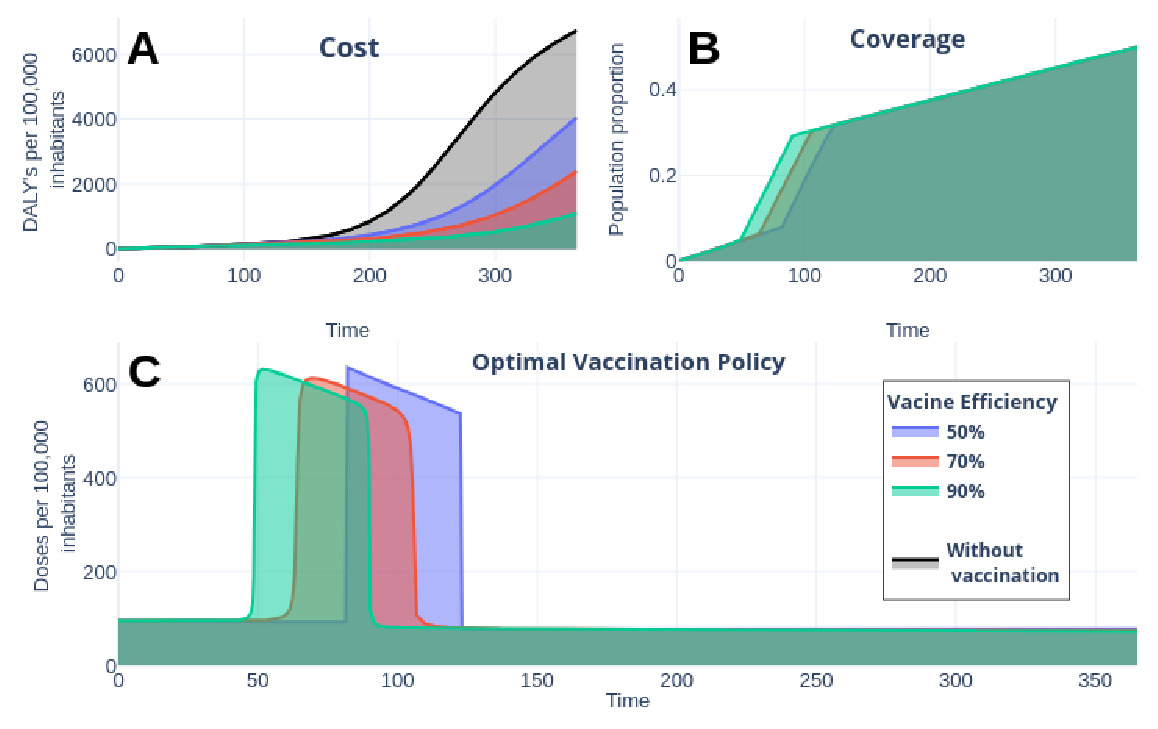
\includegraphics[scale=.6,
            keepaspectratio]{%
                ./EfficiencyVaccineProfile.png}
            \caption[Optimal Vaccination
            Policy]{
                Description panel A.
                Description panel
                B. Description Panel C,
                Implications illustrated
                https://plotly.com/~sauldiazinfante/85/
        }
            \label{fig:efficiencyvaccineprofile}
        \end{figure*}


        \begin{figure*}[htb]
            \centering
            \includegraphics[scale=.6,
            keepaspectratio]{%
            ./EfficiencyVaccineProfileOutbreak.png}
            \caption[Optimal Vaccination
            Policy]{
                Description panel A.
                Description panel B.
                Description panel C.
                Implications.
                Explain green translucent layer effect.
                illustrated}
            \label{fig:efficiencyvaccineprofileOutbreak}
        \end{figure*}

    \subsubsection*{Vaccine Induced Immunity}
%
    \begin{figure*}[htb]
        \centering
        \includegraphics[scale=0.6, keepaspectratio]{%
        InducedImmunityVaccineProfile%
        }
        \caption[
            Induced vaccine immunity
            effect.
        ]{
            Panel A description.
            Panel B description.
            Implication.
            Cite plotly chart link
            https://plotly.com/~sauldiazinfante/111/
        }
        \label{fig:inducedimmunityvaccineprofile}
    \end{figure*}
    \begin{figure*}[htb]
    \centering
    \includegraphics[scale=0.6, keepaspectratio]{%
        InducedImmunityVaccineProfileOutbreak%
    }
    \caption[
    Induced vaccine immunity
    effect.
    ]{
        Panel A description.
        Panel B description.
        Implication.
        Cite plotly chart link:
        https://plotly.com/~sauldiazinfante/123/
    }
    \label{fig:inducedimmunityvaccineprofile}
\end{figure*}

    \subsection{Natural Immunity Hypothesis}
        \begin{figure*}[tbh!]
            \centering
            \includegraphics[scale=0.6,
            keepaspectratio]{NaturalRecoveringProfile}
            \caption[Vaccine induced immunity profile.]{
                Panel A description,
                Panel B description,
                Panel C description,
                Implications.
                Plotly-cite: https://plotly.com/~sauldiazinfante/95/}
            \label{fig:naturalrecoveringprofile}
        \end{figure*}

        \begin{figure*}[tbh!]
            \centering
            \includegraphics[scale=0.6,
            keepaspectratio]{NaturalRecoveringProfileOutbreak}
            \caption[Vaccine induced immunity profile.]{Panel A description, Panel B
                description, Panel C description, Implications.
                Plotly: https://plotly.com/~sauldiazinfante/104/}
            \label{fig:naturalrecoveringprofile}
        \end{figure*}
